\section{Recording Environments} \label{sec:meth_RecordingEnvironments}

In order to utilize the raw eye tracking data described in section \ref{sec:hwds_RawDataOutput} for supervised learning, we need every sample to be labelled with its corresponding eye movement event. These labels will constitute the ground truth for model training, and its quality will therefore directly translate to the quality of the model produced, as well as the accuracy of predictions. The quality of a labelled dataset is directly tied to the method of labelling. This section will explain the environments necessary to generate perform classification in both the binary and multi-class case
In this section, I will describe the various methods used for data labelling, each with its purposes and advantages. \textit{The methods used will be compared and finally used for training a classification model.}

Survey by Forbes: Data scientists use 82\% of their time collecting, building and cleaning their data sets. 

\subsection{Static}
For binary classification, we limit the model to only classify whether a sample represents a saccade or not. As such, the labelling environment required can be limited to one where only saccades are labelled, whereas  all other samples can be directly labelled as fixations. This allows for a very simple system for data labelling, where the user is asked to manually indicate when he is adjusting his gaze point.

As described in section \ref{sec:hwds_TobiiEyeTracker5}, user blinking is represented in the data by a loss of samples for the duration of the blink. For blinks differing in periods from 10ms to 100ms, this constitutes the loss of 1 to 5 samples, in the general case. Following the periods of lost data, we can observe large amounts of noise, as the oculomotor muscles attempts to readjust the eye to its preceding point of fixation. To avoid data contamination by these events, we also instruct the user to indicate whenever he is blinking. This way, data contaminated by blinking can be removed as a post-processing operation. Since we cannot guarantee that the user fixates on the exact same point preceding and following a blink, we will split the time series on any blink-labelled sample such that the feature generator of section \ref{sec:meth_FeatureGeneration} does not operate on any sampling window that encapsulate contaminated data. 

The labelling environment is intended to run full screen on the recording monitor, and consist of a large single image as well as an on-screen button to indicate when the user is fixating somewhere on the image. The image is highly abstract and visually stimulating, chosen so there is no area of particular interest that draws the user's attention, and no blank areas where the user might struggle to find objects to fixate on. Such aspects might introduce unwanted bias in the data. A scaled-down version of the static labelling environment is shown in figure \ref{fig:meth_StaticLabellingEnv}.

\begin{figure}[h]
    \centering
    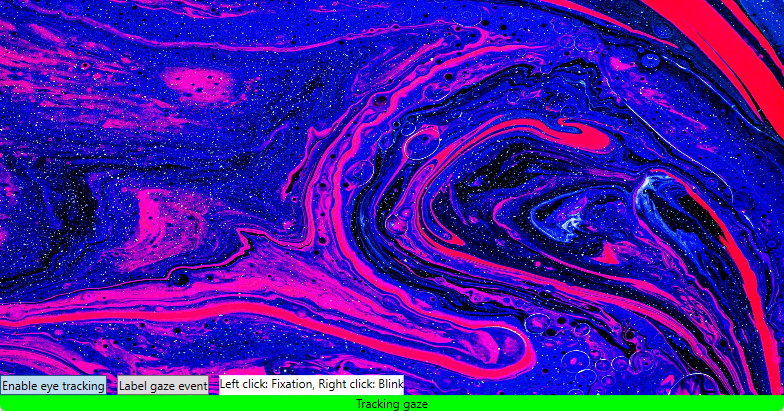
\includegraphics[width=\textwidth]{Images/Labelling/StaticEnvironment2.png}
    \caption{Static labelling environment, used to label data for the binary classification problem.}
    \label{fig:meth_StaticLabellingEnv}
\end{figure}

Unfortunately, this way of labelling data introduces bias by human error. An ideal ground truth should be impeccable in its classifications, as the machine learning classification model can never be better than the dataset from which it trains its parameters. For this reason, we introduce a manual post-labelling step, where an operator scans through the labelled samples and correct erroneous labels by observing the onset and offset of differences in recorded on-screen xy-coordinates.

\subsubsection{Post-labeling}

\subsection{Dynamic}

\begin{figure}
    \centering
    \begin{minipage}{0.5\textwidth}
        \centering
        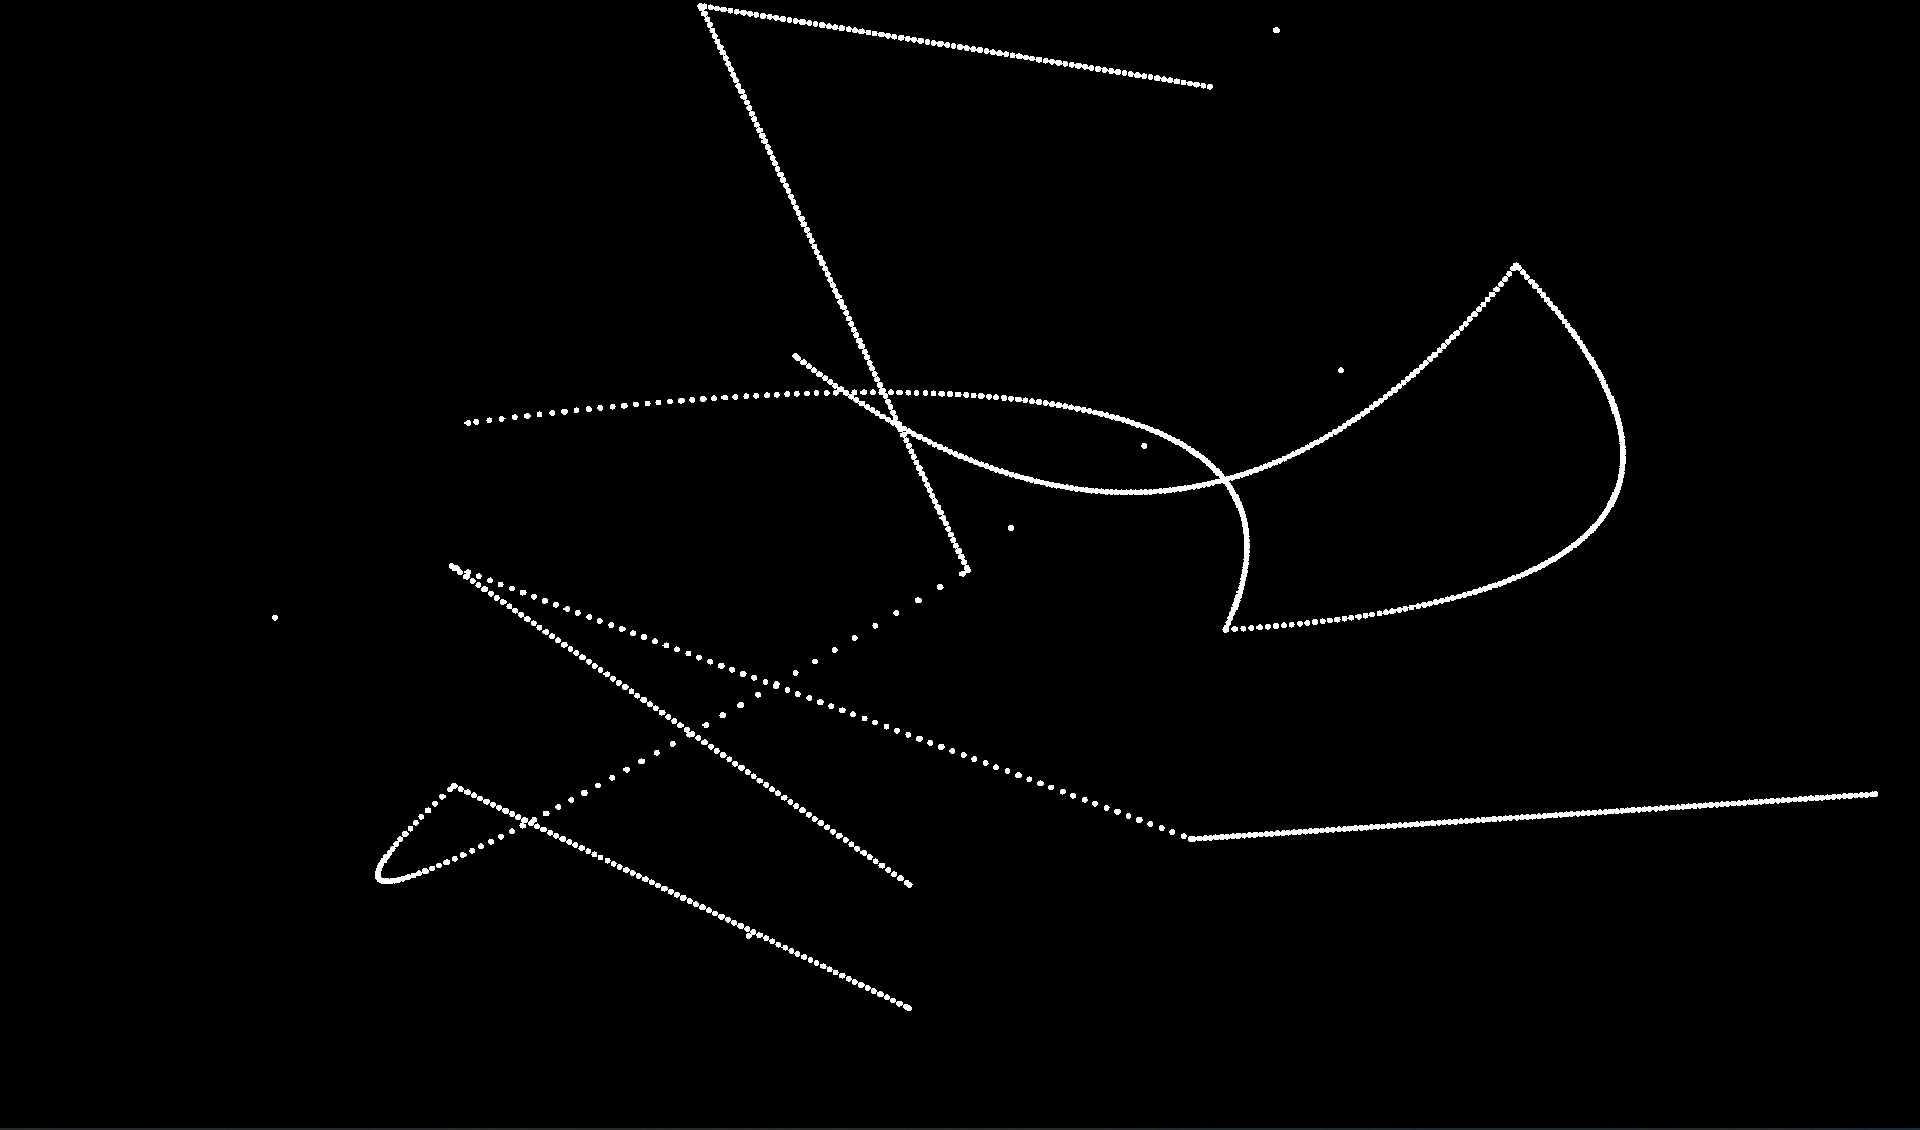
\includegraphics[width=\textwidth]{Images/Labelling/DynamicEnvScreen.png} % first figure itself
        %\caption{first figure}
    \end{minipage}\hfill
    \begin{minipage}{0.5\textwidth}
        \centering
        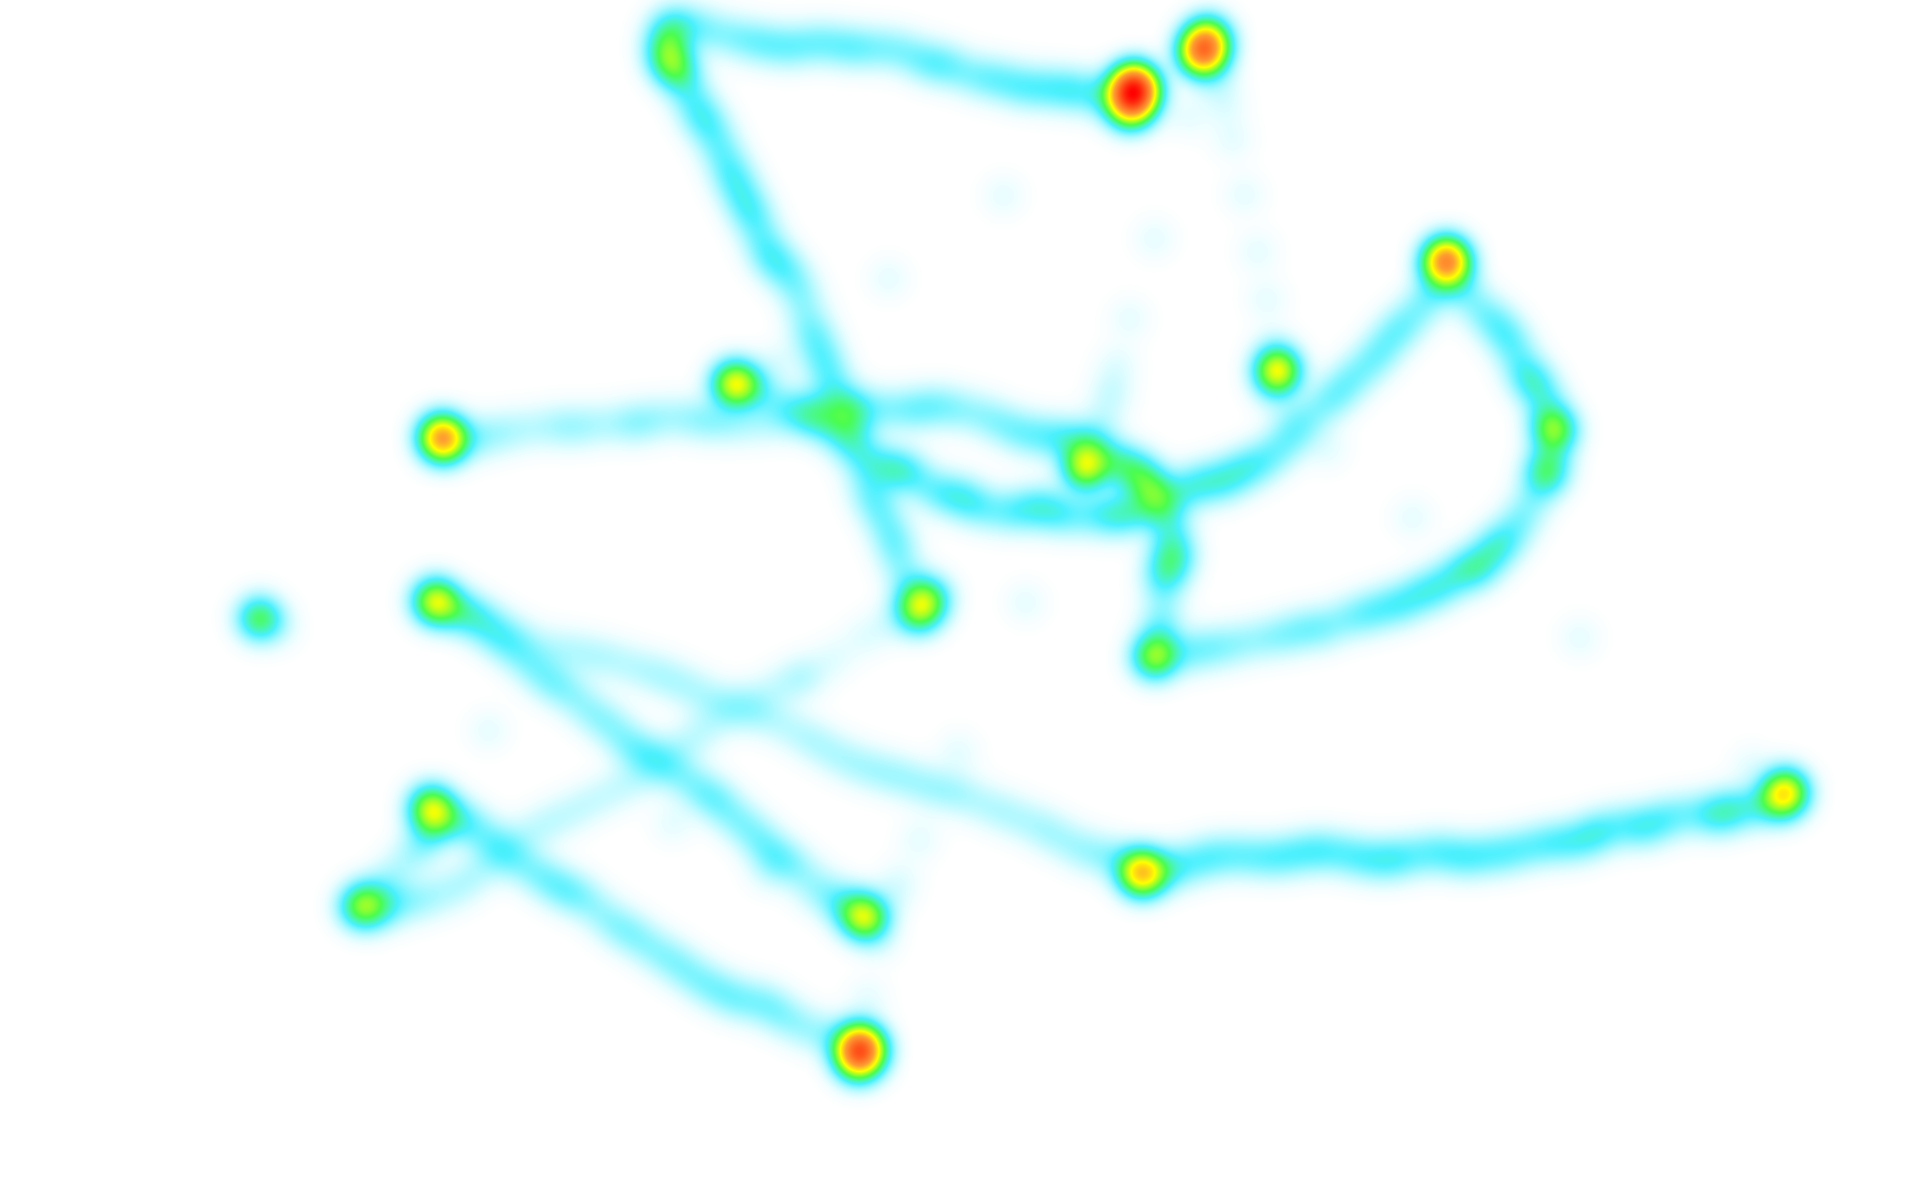
\includegraphics[width=\textwidth]{Images/Labelling/DynamicEnvHm.png}% second figure itself
        %\caption{second figure}
    \end{minipage}
    \caption{Dynamic Labelling environment. Left image represents the paths drawn by warping and moving dot during data recording. Right image is the heat map resulting from the same recording.}
    \label{fig:meth_DynamicLabellingEnv}
\end{figure}

\subsubsection{Blink Detection}

\subsubsection{Post-labeling}